\documentclass{beamer}

\usepackage{tikz}
\usetikzlibrary{shadings}
\usepackage[utf8]{inputenc}
\usepackage{amsmath,amssymb}
\usepackage[russian]{babel}
\usepackage{xcolor}
\usepackage{graphicx}
\title[]{Лабораторная работа: Численные методы вычисления интегралов}
\author[]{Веселов Фёдор, Ушаков Роман, Босенко Борис, Ежелев Георгий}

\newlength{\RightSidebarWidth} 
\setlength{\RightSidebarWidth}{1.2cm}

% используем внешний шаблон sidebar
\useoutertheme[right]{sidebar}

% убираем стандартный верхний и нижний колонтитулы
\setbeamertemplate{headline}{}
\setbeamertemplate{footline}{}

% наш вариант правой боковой панели
\setbeamertemplate{sidebar right}{%
	\begin{tikzpicture}[remember picture, overlay]
		% Можно использовать structure.fg напрямую
		\shade[top color=structure.fg!60, bottom color=structure.fg!10]
		([xshift=-2.5cm]current page.north east) rectangle (current page.south east);
		\node[anchor=center, align=center, font=\tiny, text width=2.4cm]
		at ([xshift=-1.2cm, yshift=-1.25cm]current page.north east) {
			\scriptsize \textcolor{structure.fg}{\textbf{Численное интегрирование}}\\
			\tiny Веселов Фёдор\\[0.5em]
			\tiny Ушаков Роман\\[0.5em]
			\tiny Босенко Борис\\[0.5em]
			\tiny Ежелев Георгий\\[0.5em]
		};
	\end{tikzpicture}
}

% чтобы содержимое не залезало под полосу
\setbeamersize{text margin right=\RightSidebarWidth}

\begin{document}
	\begin{frame}
		\titlepage
	\end{frame}
	
	\large \textbf{\textcolor{structure.fg}{Индивидуальная часть. Ежелев Георгий}}\\
	\begin{frame}
		\textbf{Дан интеграл функции: } \[\int_{0}^{1}  e^{-x}\]\\
		Для нахождения интеграла распишем Риманову сумму для равномерного разбиения отрезка [0;1]. Воспользуемся формулой правых прямоугольников:\\
		\[\lim_{n \to \infty}\frac{b-a}{n}*\sum_{i=1}^{n}f(x_i)\]\\
		В случае интегрирования от 0 до 1, при равномерном разбиении отрезка сумма принимает вид:\\
		\[\lim_{n \to \infty} \frac{1}{n} * \sum_{k=1}^{n} e^{-\frac{k}{n}} = I\]\\
	\end{frame}
	\begin{frame}
	\large \textbf{\textcolor{structure.fg}{Задание №2 - вычисление суммы}}\\
	Распишем по формуле суммы геометрической прогрессии:\\
	\[I = \lim_{n \to \infty} \frac{1}{n} * \frac{e^{-\frac{n}{n}} - 1 }{e^{-\frac{1}{n}} - 1} = \lim_{n \to \infty} \frac{1}{n} * \frac{e^{-1} - 1 }{e^{-\frac{1}{n}} - 1}\]\\
	Теперь воспользуемся эквивалентностью, следствием из второго замечательного предела:
	\[\lim_{x \to 0} \frac{e^{x} - 1}{x} \sim 1\]\\
	Тогда имеем:
	\[I = \lim_{n \to \infty} \frac{1}{n} * \frac{e^{-1} - 1 }{e^{-\frac{1}{n}} - 1} =\lim_{n \to \infty} \frac{1}{n} * \frac{e^{-1} - 1}{-\frac{1}{n}} = \lim_{n \to \infty} -(e^{-1} - 1) = \boxed{1 - e^{-1}}\]
	\end{frame}
	\begin{frame}
		\large \textbf{\textcolor{structure.fg}{Задание №3 - Проверка существования интеграла}}\\
	Данная функция \(e^{-x}\) интегрируема на [0,1], т.к. является непрерывной на данном отрезке, что является достаточным условием по признаку интегрируемости.\\
	\large \textbf{\textcolor{structure.fg}{Задание №4 - Проверка прямым интегрированием}}\\
	\[\int_{0}^{1}  e^{-x} = -e^{-x}\Big\vert_{0}^{1} = \boxed{1 - e^{-1}}\]\\
\end{frame}
\begin{frame}
	\large \textbf{\textcolor{structure.fg}{Часть №2 - численное интегрирование}}\\
	Задание выполнено на языке программирования Python. Для отрисовки графиков использовалась библиотека matplotlib.\\
	Значение исходного определенного интеграла: \(I = 1-\frac{1}{e} \approx 0.63212...\)\\
\end{frame}
\begin{frame}
	\large \textbf{\textcolor{structure.fg}{Метод левых прямоугольников}}\\
	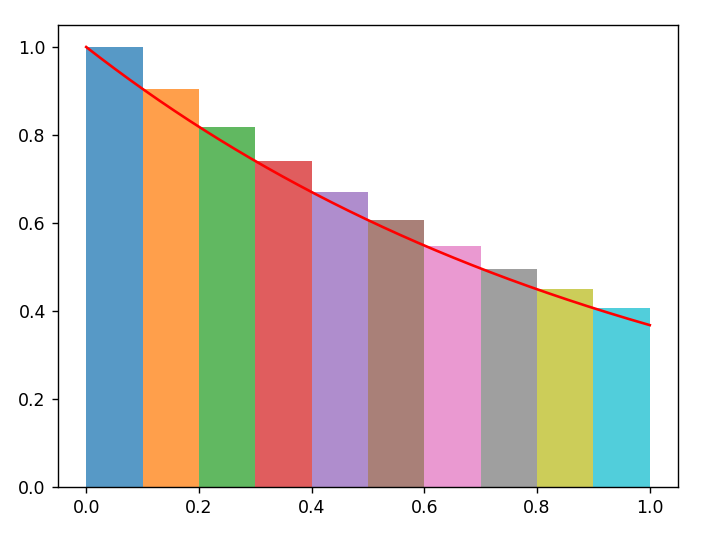
\includegraphics[width = 10cm, height = 7cm]{left_10.png}\\
	n = 10. Ранг разбиения 0.1. Результат: \(R \approx 0.66425\).\\
\end{frame}
\begin{frame}
	\large \textbf{\textcolor{structure.fg}{Метод левых прямоугольников}}\\[1cm]
	Формула погрешности:
	\[|R_n| \leq max_{x \in [a, b]} |f^\prime(x)| \frac{(b-a)^2}{2n}\]
	Тогда имеем:
	\[|R_n| \leq max_{x \in [0, 1]} |-e^{-x}| \frac{1}{2n} = \frac{1}{2n}\]
	Последнее равенство корректно в силу монотонности производной на отрезке [0, 1]\\
	При n = 10, \(|R_n| \leq 0.05\), \(|I - R|\approx 0.03213\). Т.е. погрешность рассчетов не превышает максимальную.
\end{frame}
\begin{frame}
	\large \textbf{\textcolor{structure.fg}{Метод правых прямоугольников}}\\
	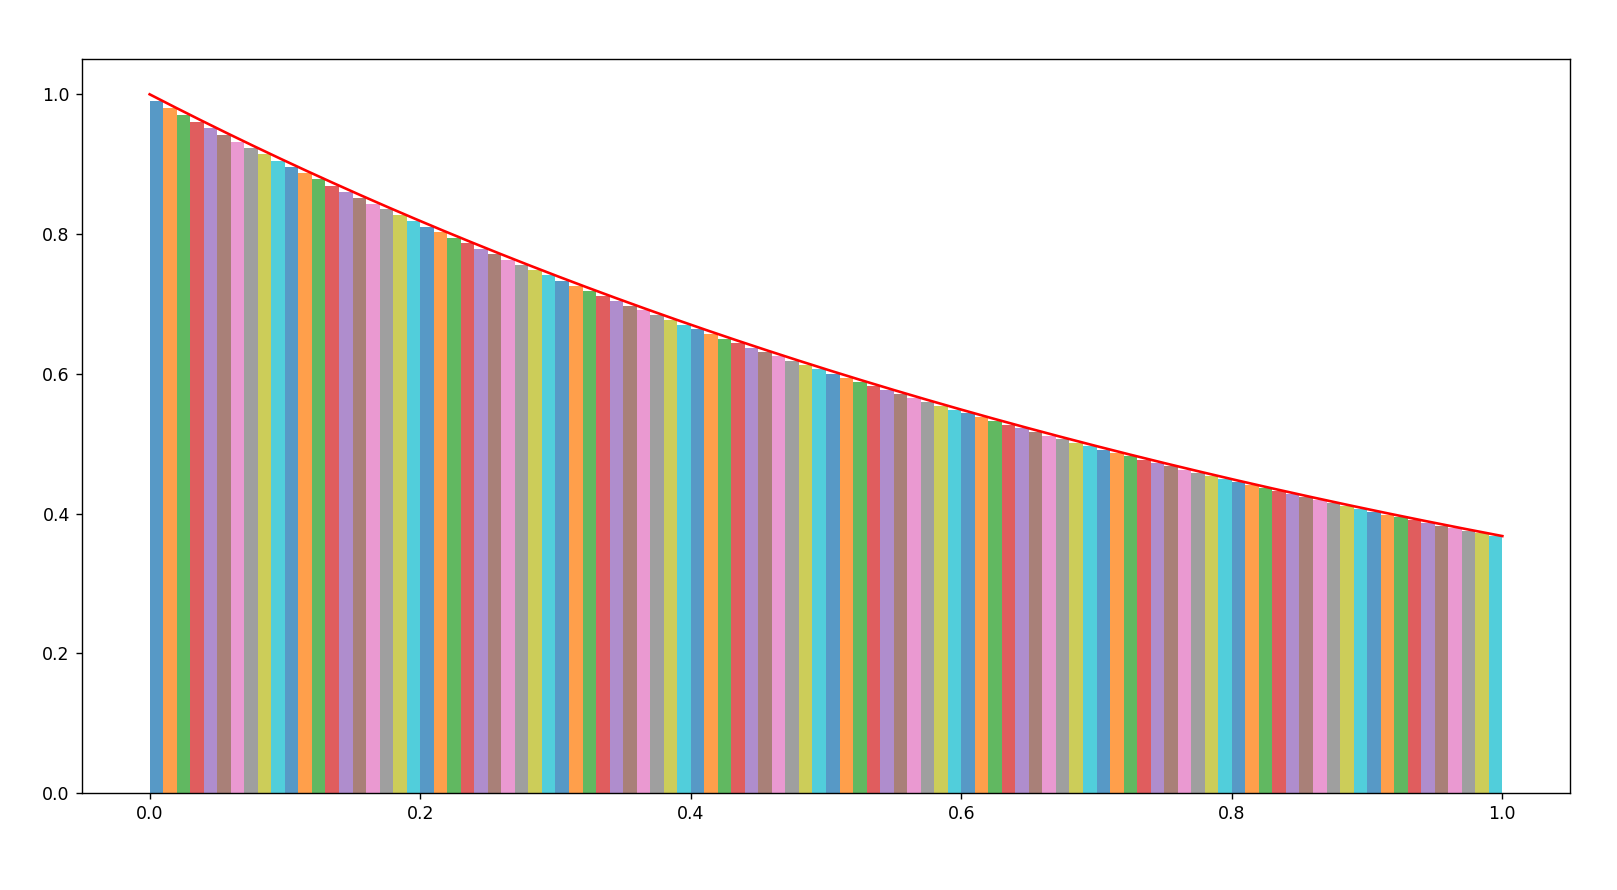
\includegraphics[width = 10cm, height = 6cm]{right_100.png}\\
	n = 100. Ранг разбиения 0.01. Результат: \(R \approx 0.62896\).
	Формула погрешности та же, что и в предыдущем методе:
	\[|R_n| \leq \frac{1}{2n}\]
	\end{frame}
	\begin{frame}
		\large \textbf{\textcolor{structure.fg}{Метод правых прямоугольников}}\\[1cm]
	При n = 100, \(|R_n| \leq 0.005\), \(|I - R|\approx 0.00316\). Т.е. погрешность рассчетов не превышает максимальную.
	\end{frame}
	\begin{frame}
		\large \textbf{\textcolor{structure.fg}{Метод трапеций}}\\
	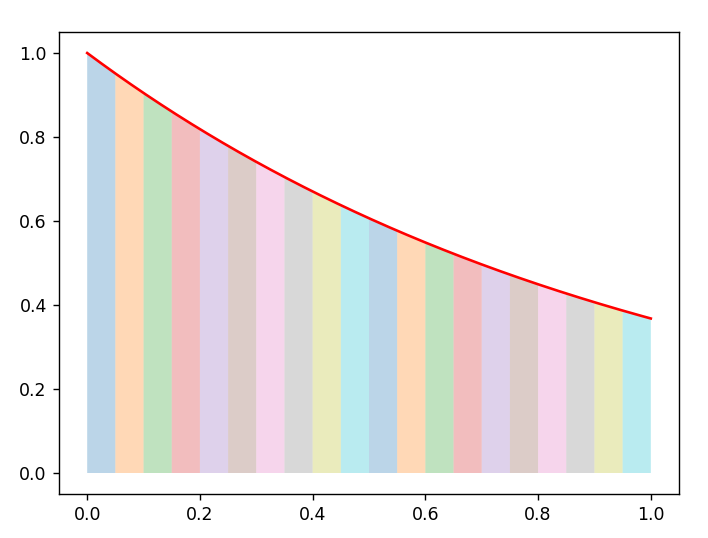
\includegraphics[width = 10cm, height = 7cm]{trap_10.png}\\
	n = 20. Ранг разбиения 0.05. Результат: \(R \approx 0.63225\).\\
\end{frame}
\begin{frame}
	\large \textbf{\textcolor{structure.fg}{Метод трапеций}}\\[1cm]
	Формула погрешности:
	\[|R_n| \leq max_{x \in [a, b]} |f^{\prime\prime}(x)| \frac{(b-a)^3}{12n^2}\]
	Тогда имеем:
	\[|R_n| \leq max_{x \in [0, 1]} |e^{-x}| \frac{1}{12n^2} = \frac{1}{12n^2}\]
	
	При n = 20, \(|R_n| \leq 0.00020...\), \(|I - R|\approx 0.00013\). Т.е. погрешность рассчетов не превышает максимальную.
	\end{frame}
	\begin{frame}
		\large \textbf{\textcolor{structure.fg}{Метод средних прямоугольников}}\\
	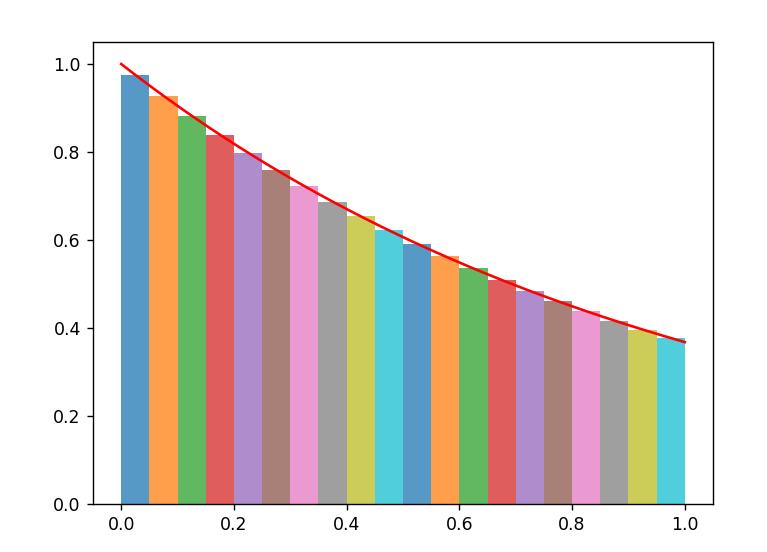
\includegraphics[width = 10cm, height = 7cm]{middle_200.png}\\
	n = 200. Ранг разбиения 0.005. Результат: \(R \approx 0.63211\).
\end{frame}
\begin{frame}
	\large \textbf{\textcolor{structure.fg}{Метод средних прямоугольников}}\\[1cm]
	Формула погрешности:
	\[|R_n| \leq max_{x \in [a, b]} |f^{\prime\prime}(x)| \frac{(b-a)^3}{24n^2}\]
	Тогда имеем:
	\[|R_n| \leq max_{x \in [0, 1]} |e^{-x}| \frac{1}{24n^2} = \frac{1}{24n^2}\]\\
	При n = 20, \(|R_n| \leq 0.00010...\), \(|I - R|\approx 0.00001\). Т.е. погрешность рассчетов не превышает максимальную.\\[1cm]
	
	Отметим, что \(e^{-x} \in C^2[0, 1]\), так что все 4 полученные оценки погрешности корректны. Для всех четырех методов выполняется: \(|R_n| \xrightarrow{n \to \infty}{} 0\).
	\end{frame}
	
	\large \textbf{\textcolor{structure.fg}{Индивидуальная часть. }}\\
			
\end{document}